\documentclass{article}
\usepackage[utf8]{inputenc}
\usepackage{enumerate}
\usepackage{amsmath}
\usepackage{amssymb}
\usepackage{amsfonts}
\usepackage{amstext}
\usepackage{amsthm}
\usepackage{mathtools}
\usepackage{tikz}
\usepackage{tikz-3dplot}
\usetikzlibrary{angles, quotes}
\usepackage{amssymb}
\usepackage{amsmath}
\usepackage{cancel}
\DeclarePairedDelimiter{\ceil}{\lceil}{\rceil}
\title{Calculus III Midterm 1 Practice}
\author{Eddie Ozuna,Tyler Franklin}

\begin{document}
\maketitle

Recall that the dot product of two vectors $\vec{u}$ and $\vec{v}$ may be denoted by any of
the expressions " $\vec{u}\cdot \vec{v}$ ", " $<\vec{u}, \vec{v}>$ ", " $\vec{u}^T \vec{v}$ ", and is also referred to as “the inner product”.
\\
\\
The cross product of two vectors u and v will be denoted “ $\vec{u}\times\vec{v}$ ”.
Also, recall that the length of any vector $\vec{u}$ is denoted by $\mid\vec{u}\mid$.
\\
\\
Throughout this review, lets establish the following notation:\\
\\
\\
$\vec{u}=\left(\!\begin{array}{c}u_{1} \\ u_{2} \\  u_{3}\end{array} \!\right)$,
$\vec{v}=\left(\!\begin{array}{c}v_{1} \\ v_{2} \\  v_{3}\end{array} \!\right)$,
$\vec{w}=\left(\!\begin{array}{c}w_{1} \\ w_{2} \\  w_{3}\end{array} \!\right)$
\\
\\
\\
$e_{1}=\left(\!\begin{array}{c}1 \\ 0 \\  0\end{array} \!\right)$,
$e_{2}=\left(\!\begin{array}{c}0 \\ 1 \\  0\end{array} \!\right)$,
$e_{3}=\left(\!\begin{array}{c}0 \\ 0 \\  1\end{array} \!\right)$
\\
\\
\\
\begin{enumerate}[1.]
	\item\textbf{Prove that for any two vectors u and v, the inner product of u and v is equal to $\mid\vec{u}\mid\mid\vec{v}\mid\cos(\theta)$ where $\theta$ is the angle between $\vec{u}$ and $\vec{v}$.\\\\Hint: Draw the picture and recall the Law of Cosines is just a degeneration of
	      the Pythagorean Theorem:}\\
	\\
	Derivation: Law of Cosine\\
	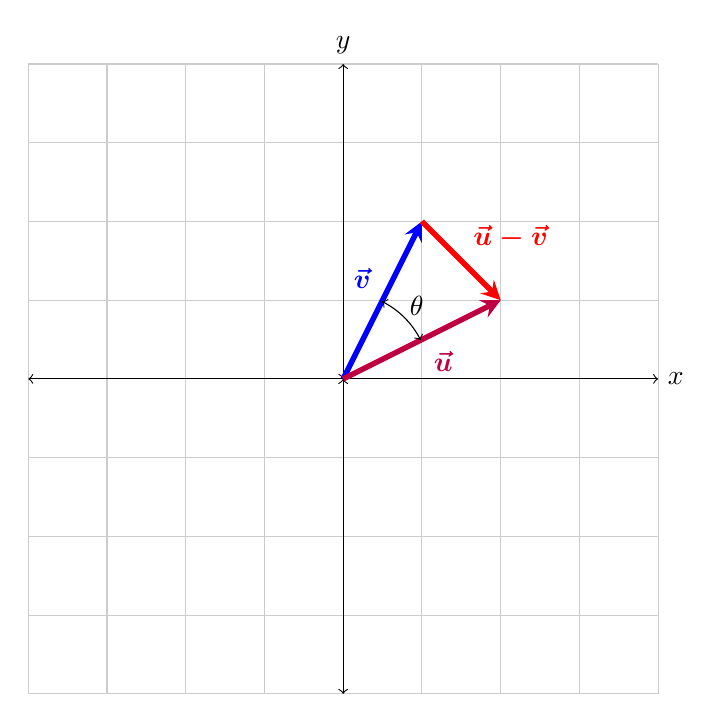
\begin{tikzpicture}
		\draw[thin,gray!40] (-4,-4) coordinate (o) grid (4,4);
		\draw[<->] (0,0)--(0,0) coordinate (o) node[right]{};
		\draw[<->] (-4,0)--(4,0)  node[right]{$x$};
		\draw[<->] (0,-4)--(0,4)  node[above]{$y$};
		\draw[line width=2pt,blue,-stealth](0,0)--(1,2) coordinate (x) node[midway,auto]{$\boldsymbol{\vec{v}}$};
		\draw[line width=2pt,purple,-stealth](0,0)--(2,1) coordinate (y) node[midway,auto,swap]{$\boldsymbol{\vec{u}}$};
		\draw[line width=2pt,red,-stealth](1,2)--(2,1) node[midway,auto]{$\boldsymbol{\vec{u}-\vec{v}}$};
		\pic [draw, <->,
			angle radius=11mm, angle eccentricity=1.2,
		"$\theta$"] {angle = y--o--x};
	\end{tikzpicture}\\
	$\mid\vec{u}-\vec{v}\mid^{2} = \mid\vec{u}\mid^{2} + \mid\vec{v}\mid^{2}-\hspace{.1cm}2\mid\vec{u}\mid\cdot\mid\vec{v}\mid\cos(\theta)$\\
	\\
	$\cancel{\mid\vec{u}\mid^{2}}-\hspace{.1cm}2\vec{v}\cdot\vec{u}\hspace{.1cm}+\cancel{\mid\vec{v}\mid^{2}}=\cancel{\mid\vec{u}\mid^{2}} + \cancel{\mid\vec{v}\mid^{2}}-2\mid\vec{u}\mid\cdot\mid\vec{v}\mid\cos(\theta)$\\
	\\
	$\cancel{-2}\vec{v}\cdot\vec{u} = \cancel{-2}\mid\vec{u}\mid\cdot\mid\vec{v}\mid\cos(\theta)$\\
	\\
	$\vec{v}\cdot\vec{u} = \mid\vec{u}\mid\cdot\mid\vec{v}\mid\cos(\theta)$\\
\end{enumerate}
\begin{enumerate}[2.]
	\item\textbf{Are the vectors $\vec{u}=\left(\!\begin{array}{c}1 \\ 2 \\  3\end{array} \!\right)$ , $\vec{v}=\left(\!\begin{array}{c}-2 \\ 1 \\  0\end{array} \!\right)$ orthogonal? Why or why not?}\\
	\\
	Vectors are orthogonal(perpendicular) if and only if the result of the dot product is zero.\\
	\\
	($\vec{u}\cdot\vec{v})=(1\cdot-2)+(2\cdot1)+(3\cdot0)=0$
	\\
	\\
	Yes they are orthogonal 
\end{enumerate}
\begin{enumerate}[3.]
	\item\textbf{Prove that the cross product of two vectors $\vec{u}$ and $\vec{v}$ is actually orthogonal to each of $\vec{u}$ and $\vec{v}$ simultaneously, i.e. $\vec{u}\times\vec{v}$ is orthogonal to $\vec{u}$ and $\vec{u}\times\vec{v}$ is
	      orthogonal to $\vec{v}$ }
	\\
	\\
	Step 1. Take the cross product of $\vec{u}$ and $\vec{v}$\\
	\\
	$\vec{u}\times\vec{v}=\begin{vmatrix}
	\hat{i}&\hat{j}&\hat{k}\\
	u_{1}&u_{2}&u_{3}\\
	v_{1}&v_{2}&v_{3}\\
	\end{vmatrix}=\hat{i}
	\begin{vmatrix}
		u_{2} & u_{3} \\
		v_{2} & v_{3} \\
	\end{vmatrix}-\hat{j}\begin{vmatrix}
	u_{1}&u_{3}\\
	v_{1}&v_{3}\\
	\end{vmatrix}+\hat{k}\begin{vmatrix}
	u_{1}&u_{2}\\
	v_{1}&v_{2}\\
	\end{vmatrix}\\
	=\hat{i}(u_{2}v_{3}-u_{3}v_{2})-\hat{j}(u_{1}v_{3}-u_{3}v_{1})+\hat{k}(u_{1}v_{2}-u_{2}v_{1})$\\
	\\
	Let define $\vec{w}$ to be equal to the result of the cross product of $\vec{u}$ and $\vec{v}$\\
	\\
	Step 2. From our previous knowledge we know that if the result of the dot product is zero the vectors are orthogonal(perpendicular). With that being said let perform the dot products of vector $\vec{u}$ with $\vec{w}$ and $\vec{v}$ with $\vec{w}$.\\
	\\
	$\vec{w} = <(u_{2}v_{3}-u_{3}v_{2}),-(u_{1}v_{3}-u_{3}v_{1}),(u_{1}v_{2}-u_{2}v_{1})>$\\
	\\
	$\vec{u}\cdot\vec{w}=u_{1}(u_{2}v_{3}-u_{3}v_{2})-u_{2}(u_{1}v_{3}-u_{3}v_{1})+u_{3}(u_{1}v_{2}-u_{2}v_{1})\\=u_{1}u_{2}v_{3}-u_{1}v_{2}u_{3}-u_{1}u_{2}v_{3}+v_{1}u_{2}u_{3}+u_{1}u_{3}v_{2}-v_{1}u_{2}u_{3}=0$\\
	\\ 
	$\vec{v}\cdot\vec{w}=v_{1}(u_{2}v_{3}-u_{3}v_{2})-v_{2}(u_{1}v_{3}-u_{3}v_{1})+v_{3}(u_{1}v_{2}-u_{2}v_{1})\\=v_{1}u_{2}v_{3}-v_{1}v_{2}u_{3}-u_{1}v_{2}v_{3}+v_{1}v_{2}u_{3}+u_{1}v_{2}v_{3}-v_{1}u_{2}v_{3}=0$\\
	\\
	Proven Both yield a result of zero which state they are orthogonal(perpendicular) simultaneously.
\end{enumerate}
\begin{enumerate}[4.]
	\item\textbf{Find a vector that is orthogonal to each of the vectors $1\cdot e_{1}+1\cdot e_{2}+1\cdot e_{3}$ and $1\cdot e_{1}+1\cdot e_{2}+0\cdot e_{3}$. Prove that your vector is actually perpendicular to
	      each of $e_{1}$ and $e_{2}$ simultaneously}\\
	\\
	Step 1. Simplify $1\cdot e_{1}+1\cdot e_{2}+1\cdot e_{3}$ and $1\cdot e_{1}+1\cdot e_{2}+0\cdot e_{3}$.\\
	\\
	$1\cdot e_{1}+1\cdot e_{2}+1\cdot e_{3}=1\cdot<1,0,0>+1\cdot<0,1,0>+1\cdot<0,0,1>\\=<1\cdot1,1\cdot0,1\cdot0>+<1\cdot0,1\cdot1,1\cdot0>+<1\cdot0,1\cdot0,1\cdot1>\\=<1,0,0>+<0,1,0>+<0,0,1>\\=<1+0+0,0+1+0,0+0+1>=<1,1,1>$\\
	\\
	$1\cdot e_{1}+1\cdot e_{2}+0\cdot e_{3}=1\cdot<1,0,0>+1\cdot<0,1,0>+0\cdot<0,0,1>\\=<1\cdot1,1\cdot0,1\cdot0>+<1\cdot0,1\cdot1,1\cdot0>+<0\cdot0,0\cdot0,0\cdot1>\\=<1,0,0>+<0,1,0>+<0,0,0>\\=<1+0+0,0+1+0,0+0+0>=<1,1,0>$
	
	Let $\vec{p}$ and $\vec{q}$ equal to the result we got.\\
	\\
	$\vec{p}=<1,1,1>$
	\\
	$\vec{q}=<1,1,0>$\\
	\\
	Step 2. Take the cross product of vector $\vec{p}$ with $\vec{q}$\\
	\\
	$\vec{p}\times\vec{q}=\begin{vmatrix}
	\hat{i}&\hat{j}&\hat{k}\\
	1&1&1\\
	1&1&0\\
	\end{vmatrix}=\hat{i}
	\begin{vmatrix}
		1 & 1 \\
		1 & 0 \\
	\end{vmatrix}-\hat{j}\begin{vmatrix}
	1&1\\
	1&0\\
	\end{vmatrix}+\hat{k}\begin{vmatrix}
	1&1\\
	1&1\\
	\end{vmatrix}\\=\hat{i}(1\cdot0-1\cdot1)-\hat{j}(1\cdot0-1\cdot1)+\hat{i}(1\cdot1-1\cdot1)=-1\hat{i}+1\hat{j}+0\hat{k}$\\
	\\
	Let $\vec{r}$ equal to the result we got.\\
	\\
	$\vec{r} = <-1,1,0>$\\
	\\
	Step 3. Take the dot product of $\vec{e_{1}}$ with $\vec{r}$  and $\vec{e_{2}}$ with $\vec{r}$ to see if they are orthogonal simultaneously\\
	\\
	$\vec{e_{1}}\cdot\vec{r}=(1\cdot-1)+(1\cdot1)+(1\cdot0)=0$
	\\
	\\
	$\vec{e_{2}}\cdot\vec{r}=(1\cdot-1)+(1\cdot1)+(0\cdot0)=0$
	\\
	\\
	Proven Both yield a result of zero which state they are orthogonal(perpendicular) simultaneously.
\end{enumerate}
\begin{enumerate}[5.]
	\item
	      Recall that the volume of the parallelopiped (three-dimensional analogue of
	      a parallelogram) spanned by three vectors $\vec{u}$, $\vec{v}$ and $\vec{w}$ is given by:\\
	      \\
	      $<\vec{u}\times\vec{v},\vec{w}>$\\
	      \\ This just mean take the cross product of $\vec{u}$ with $\vec{v}$ and then take the dot product of the result with $\vec{w}$.\\
	      \\
	      This is known as the triple product of $\vec{u}$, $\vec{v}$ and $\vec{w}$. Interestingly enough, this is a way of defining the determinant of a matrix. Given a matrix:\\
	      \\
	      $M:=\begin{vmatrix}
	      u_{1}&v_{1}&w_{1}\\
	      u_{2}&v_{2}&w_{2}\\
	      u_{3}&v_{3}&w_{3}\\
	\end{vmatrix}$\\
	\\
	where we notice that the columns of the matrix are precisely the vectors $\vec{u}$, $\vec{v}$ and $\vec{w}$. we can actually define the determinant of the matrix M via:\\
	\\
	$det(M ) := <\vec{u}\times\vec{v},\vec{w}>$\\
	\\
	\textbf{Prove that these two definitions yield the same thing! The determinant of a
		matrix is said to encode the amount that the unit parallelopiped is scaled upon
		applying the linear transformation of space represented by the matrix.}\\
	\\
	To prove this we just need to take the determinant of M which is the left side of the equation and them evaluate the right side of the question which just mean take the cross product of $\vec{u}$ with $\vec{v}$ and then take the dot product of the result with $\vec{w}$.\\
	\\
	Left side of the equation:\\
	\\
	$det(M ) := \begin{vmatrix}
	u_{1}&v_{1}&w_{1}\\
	u_{2}&v_{2}&w_{2}\\
	u_{3}&v_{3}&w_{3}\\
	\end{vmatrix}=u_{1}\begin{vmatrix}
	v_{2}&w_{2}\\
	v_{3}&w_{3}\\
	\end{vmatrix}-v_{1}\begin{vmatrix}
	u_{2}&w_{2}\\
	u_{3}&w_{3}\\
	\end{vmatrix}+w_{1}\begin{vmatrix}
	u_{2}&v_{2}\\
	u_{3}&v_{3}\\
	\end{vmatrix}\\\\:=u_{1}(v_{2}w_{3} - w_{2}v_{3}) - v_{1}(u_{2}w_{3}-w_{2}u_{3})+w_{1}(u_{2}v_{3}-v_{2}u_{3})\\:=u_{1}v_{2}w_{3} - u_{1}w_{2}v_{3}-v_{1}u_{2}w_{3}+v_{1}w_{2}u_{3}+w_{1}u_{2}v_{3}-w_{1}v_{2}u_{3}$\\
	\\
	\\
	Right side of the equation:\\
	\\
	$<\vec{u}\times\vec{v},\vec{w}>$\\
	\\
	$\vec{u}\times\vec{v}=\begin{vmatrix}
	\hat{i}&\hat{j}&\hat{k}\\
	u_{1}&u_{2}&u_{3}\\
	v_{1}&v_{2}&v_{3}\\
	\end{vmatrix}=\hat{i}
	\begin{vmatrix}
		u_{2} & u_{3} \\
		v_{2} & v_{3} \\
	\end{vmatrix}-\hat{j}\begin{vmatrix}
	u_{1}&u_{3}\\
	v_{1}&v_{3}\\
	\end{vmatrix}+\hat{k}\begin{vmatrix}
	u_{1}&u_{2}\\
	v_{1}&v_{2}\\
	\end{vmatrix}\\
	=\hat{i}(u_{2}v_{3}-u_{3}v_{2})-\hat{j}(u_{1}v_{3}-u_{3}v_{1})+\hat{k}(u_{1}v_{2}-u_{2}v_{1})$\\
	\\
	$<\vec{u}\times\vec{v},\vec{w}> := w_{1}(u_{2}v_{3}-u_{3}v_{2})-w_{2}(u_{1}v_{3}-u_{3}v_{1})+w_{3}(u_{1}v_{2}-u_{2}v_{1})\\:=w_{1}u_{2}v_{3}-w_{1}u_{3}v_{2}-w_{2}u_{1}v_{3}+w_{2}u_{3}v_{1}+w_{3}u_{1}v_{2}-w_{3}u_{2}v_{1}$\\
	\\
	You can clearly see that they are equal to each other proven!
\end{enumerate}
\begin{enumerate}[6.]
	\item\textbf{The twisted cubic curve is parametrized by a single parameter t via:\\$t\mapsto\left(\!\begin{array}{c}x(t) = t \\ y(t)=t^{2} \\  z(t)=t^{3}\end{array} \!\right)$\\\\Find the parametrization of the tangent vector to the twisted cubic curve. Use your parametrization of the tangent vector to find a vector perpendicular to the twisted cubic curve at the point$\left(\!\begin{array}{c}1 \\ 1 \\  1\end{array} \!\right)$ on the curve.}
	\\
	\\
	Let $c(t)=\left(\!\begin{array}{c}x(t) = t \\ y(t)=t^{2} \\  z(t)=t^{3}\end{array} \!\right)$
	\\
	\\
	Step 1. Take the derivative of c(t)\\
	\\
	c'(t)=$\left(\!\begin{array}{c}x(t) = 1 \\ y(t)= 2t \\  z(t)=3t^{2}\end{array} \!\right)$\\
	\\
	Step 2. Now find the tangent vector at the point $\left(\!\begin{array}{c}1 \\ 1 \\  1\end{array} \!\right)$\\
	\\
	c'(t) = $\left(\!\begin{array}{c} 1 \\ 2 \\  3\end{array} \!\right)$\\
	\\
	\\
	Step 3. Find any vector that will give zero after taken the dot product with vector $<1,2,3>$\\
	\\
	Vector $<-2,1,0>$ will work \\
	\\
	$<-2,1,0>\cdot<1,2,3>=(-2\cdot1)+(1\cdot2)+(0\cdot3)=0$ 
\end{enumerate}
\begin{enumerate}[7.]
	\item\textbf{Recall that the determinant of a matrix is said to encode the amount that the
	      unit parallelopiped is scaled upon applying the linear transformation of space
	      represented by the matrix. Consider the linear transformation described by\\\\$\left(\!\begin{array}{c}\vec{e_{1}}\mapsto2\cdot\vec{e_{1}}\\ \vec{e_{2}}\mapsto2\cdot\vec{e_{2}} \\  \vec{e_{3}}\mapsto2\cdot\vec{e_{3}}\end{array} \!\right)$\\which maps each of $\vec{e_{1}}$ , $\vec{e_{2}}$  , and $\vec{e_{3}}$  to twice themselves. The matrix representing
	      this linear transformation is\\\\$\left(\!
	      \begin{array}{c}
	      	2 \hspace{.5cm} 0 \hspace{.5cm} 0 \\
	      	0 \hspace{.5cm} 2 \hspace{.5cm} 0 \\
	      	0 \hspace{.5cm} 0 \hspace{.5cm} 2 \\
	      \end{array}
	      \!\right)$\\\\\\Notice that the columns of this matrix are exactly the images 2 · $\vec{e_{1}}$ , 2 · $\vec{e_{2}}$ , and 2 · $\vec{e_{3}}$ of each of $\vec{e_{1}}$ , $\vec{e_{2}}$ , and $\vec{e_{3}}$ . Draw the “before and after” picture of
	      what three-dimensional space looks like before applying the transfor-
	      mation, and then what it looks like after applying the transformation.
	      What happens to the unit cube spanned by the vectors $\vec{e_{1}}$ , $\vec{e_{2}}$ , and $\vec{e_{3}}$ ?
	      Of course, the volume of the original unit cube is 1 · 1 · 1 = 1. What is the vol-
	      ume of the resulting parallelopiped? Verify that the volume changes
	      by the amount you say by computing the determinant of the matrix
	      representing the transformation of space and demonstrating that it
	equals the number you said.}
\end{enumerate}
\begin{enumerate}[8.]
	\item\textbf{Find the equation of the plane that is tangent to the surface embedded
	      in $\mathbb{R}^{3}$ that is the graph of the function $f(x,y):= x^{2}+y^{2}$ at the point$\left(\!\begin{array}{c}1 \\ 2\\  1^{2}+2^{2}\end{array} \!\right)$.}\\
	\\
	\\
	Step 1. Find the Gradient Vector by taking the partial derivative of the function $f(x,y):= x^{2}+y^{2}$\\
	\\
	$\nabla(f(x,y))= \left(\!\begin{array}{c}\frac{\partial f}{\partial x} \\\frac{\partial f}{\partial y}\end{array} \!\right)=\left(\!\begin{array}{c}2x \\\ 2y \end{array} \!\right)$\\
	\\
	$\nabla(f(1,2))=\left(\!\begin{array}{c}2 \\\ 4 \end{array} \!\right)$\\
	\\
	\\
	where a = 2 and b = 4 and c = -1
	\\
	\\
	Step 2. General form of a equation of a plane a(x-$x_{0}$)+b(y-$y_{0}$)+c(z-$z_{0}$)=0\\
	\\
	2(x-1)+4(y-2)-1(z-5)=0
\end{enumerate}
\begin{enumerate}[9.]
	\item\textbf{In how many ways can two lines intersect in three-dimensional space? Draw
	      all of the ways and provide examples.
	      Recall that in two-dimensional space, two lines with different slopes must inter-
	      sect. In three-dimensional space, is this still true? If so, prove it. Else, provide
	      an explicit counterexample.
	      In how many ways can two planes intersect in three-dimensional space? Draw
	all of the ways and provide examples}
\end{enumerate}
\begin{enumerate}[10.]
	\item\textbf{Find an equation of a plane whose intersection with the cone defined by the
	      equation\\\\$x^{2} + y^{2} = z^{2}$\\\\resembles a parabola justifying the parabola’s description as a conic section. Verify that your choice of plane has the appropriate intersection with the cone by demonstrating that the solution set of the equation defining the cone and your plane is actually that of a parabola.}\\
	\\
	Step 1. let $f(x,y,z)=x^{2} + y^{2}- z^{2}$ and take the partial derivative\\
	\\
	$f'(x,y,z)=2x+2y-2z$\\
	\\
	Step 2. General form of a equation of a plane a(x-$x_{0}$)+b(y-$y_{0}$)+c(z-$z_{0}$)=0\\
	\\
	Let a=2 b=2 c=-2
\end{enumerate}
\begin{enumerate}[11.]
	\item\textbf{At which point will the tangent plane to the cone described by $xy = z^2$
	be ill-defined? Can you explain why? What does this surface look like?}
\end{enumerate}
\begin{enumerate}[12.]
	\item\textbf{Calculate the directional derivative of the function $f(x, y) := x^2-y^2$ at the point $p := \left(\!\begin{array}{c} 2 \\\ 1 \end{array} \!\right)$ in the direction of the (unit) vector parallel to $v := \left(\!\begin{array}{c} 1 \\\ 0 \end{array} \!\right)$ using the limit definition. Then, calculate the inner product\\
	      \\
	      $<\nabla(f(x,y)),v>$\\\\and verify that it is equal to the result acquired using the limit definition of the directional derivative of f at p in the direction of v}\\
	\\
	Step 1. Calculate the directional derivative using the limit definition\\
	\\
	$D_{u}f(\vec{p})=\lim_{h \to 0} \frac{f(\vec{p}+h\cdot\vec{u})-f(\vec{p})}{h}$\\
	\\
	$D_{u}f(<2,1>)=\lim_{h \to 0} \frac{f(<2,1>+h\cdot<1,0>)-f(<2,1>)}{h}$\\
	\\
	$=\lim_{h \to 0} \frac{f(<2,1>+<h,0>)-f(<2,1>)}{h}$\\
	\\
	$=\lim_{h \to 0} \frac{f(<2+h,1+0>)-f(<2,1>)}{h}$\\
	\\
	$=\lim_{h \to 0} \frac{(2+h)^{2}-1^{2}-(2^{2}-1^{2})}{h}$\\
	\\
	$=\lim_{h \to 0} \frac{4+4h+h^{2}-4}{h}$\\
	\\
	$=\lim_{h \to 0} \frac{4h+h^{2}}{h}$\\
	\\
	$=\lim_{h \to 0} \frac{h(4+h)}{h}$
	$=\lim_{h \to 0} (4+h)=4$
	\\
	\\
	Step 2. Calculate the inner product which just mean the dot product using $<\nabla(f(x,y)),v>$
	\\
	\\
	$\nabla(f(x,y)=<2x,-2y>$\\
	$\nabla(f(2,1)=<2x,-2y>=<4,-2>$\\
	\\
	$<(4,-2),(1,0)>=(4\cdot1)+(-2\cdot0)=4$
	\\
	\\
	They are both equal 
\end{enumerate}
\begin{enumerate}[13.]
	\item\textbf{Find the normal vector to the surface defined by the equation $x^{2} + y^{2} + z^{2} =1^{2}$ at the point $v := \left(\!\begin{array}{c} \frac{3}{5}\\ \frac{4}{5} \\ 0 \end{array} \!\right)$ and use this normal vector to find the equation of the plane tangent to the surface at this point.}\\
	\\
	Step 1. Let $f(x,y,z)=x^{2} + y^{2} + z^{2} -1^{2}$ and calculate the gradient vector\\
	\\
	$\nabla(f(x,y,z)=<2x,2y,2z>$\\
	\\
	$\nabla(f(\frac{3}{5},\frac{4}{5},0)=<\frac{6}{5},\frac{8}{5},0>$\\
	\\
	Step 2. General form of a equation of a plane a(x-$x_{0}$)+b(y-$y_{0}$)+c(z-$z_{0}$)=0\\
	\\
	$a=\frac{6}{5}$ $b=\frac{8}{5}$ $c=0$\\
	\\
	$\frac{6}{5}(x-\frac{3}{5})+\frac{8}{5}(y-\frac{4}{5})+0(z-0)=0$
\end{enumerate}
\begin{enumerate}[14.]
	\item\textbf{Find all extrema of the 
	      function $f(x,y) := 3x^{2}y+y^{3}-2x^{2}-2y^{2}+3$. In what direction from $\left(\!\begin{array}{c} 0 \\ 0 \\ 3 \end{array} \!\right)$should we travel to ascend most quickly? descend most quickly? How do you know?}\\
	\\
	Reminder: $D(a,b)= \begin{vmatrix}
	\frac{\partial{f^{2}}}{\partial{x^{2}}}&\frac{\partial{f}}{\partial{y}}(\frac{\partial{f}}{\partial{x}})\\\\
	\frac{\partial{f}}{\partial{x}}(\frac{\partial{f}}{\partial{y}})&\frac{\partial{f^{2}}}{\partial{y^{2}}}\\\\
	\end{vmatrix} = 0 \mapsto  undefined$ \\ 
	\\
	$\hspace{10cm}< 0\mapsto$ Saddle point\\
	\\
	$\hspace{10cm}> 0\mapsto$ We need to use the second partial derivative to respect to x to find out whether is a local minimum or maximum. \\
	\\
	
	Step 1. Take the partial derivative of $f(x,y) := 3x^{2}y+y^{3}-2x^{2}-2y^{2}+3$ to respect to x and y. Also, Take the second partial derivative to respect to x and y. Also, take the partial derivative of the partial derivative of y to respect to x and take the partial derivative of the partial derivative of x to respect to y.
	\\
	\\
	$\frac{\partial{f}}{\partial{x}}=6xy-4x$          \hspace{2.9cm}$\frac{\partial{f^{2}}}{\partial{x^{2}}}=6y-4$\\
	\\
	$\frac{\partial{f}}{\partial{y}}=3x^{2}+3y^{2}-4y$ \hspace{2cm}$\frac{\partial{f^{2}}}{\partial{y^{2}}}=6y-4$\\
	\\
	$\frac{\partial{f}}{\partial{x}}(\frac{\partial{f}}{\partial{y}})=6x$\\
	\\
	$\frac{\partial{f}}{\partial{y}}(\frac{\partial{f}}{\partial{x}})=6x$ \\
	\\
	Step 2. Calculate the critical points by setting $\frac{\partial{f}}{\partial{x}}=0$ and $\frac{\partial{f}}{\partial{y}}=0$. Solve the simultaneous equations.\\
	\\
	$6xy-4x=0$\\
	$3x^{2}+3y^{2}-4y=0$
	\\
	\\
	$6xy-4x=0\\6xy=4x\\y=\frac{4x}{6x}=\frac{4}{6}=\frac{2}{3}$\\
	$y=\frac{2}{3}$\\
	\\
	Plug in $y=\frac{2}{3}$ in equation $3x^{2}+3y^{2}-4y=0$\\
	\\
	\\$ 3(x)^{2}+3(\frac{2}{3})^{2}-4(\frac{2}{3})=0 \\ 3(x)^{2}+(\frac{4}{3})-\frac{8}{3}=0\\ \\ 3(x)^{2}-\frac{4}{3}=0 \\ 3(x)^{2}=\frac{4}{3} \\ x^{2}=\frac{4}{9} \\ \\ x=\frac{2}{3}$ or $x=-\frac{2}{3}$ \\
	\\
	Critical points: $(\frac{2}{3},\frac{2}{3})$ and $(-\frac{2}{3},\frac{2}{3})$
	\\
	\\
	Step 3. Find out if it local maximum or minimum or a saddle point by using \\\\ $D(x,y)= \begin{vmatrix}
	\frac{\partial{f^{2}}}{\partial{x^{2}}}(x,y)&\frac{\partial{f}}{\partial{y}}(\frac{\partial{f}}{\partial{x}})(x,y)\\\\
	\frac{\partial{f}}{\partial{x}}(\frac{\partial{f}}{\partial{y}})(x,y)&\frac{\partial{f^{2}}}{\partial{y^{2}}}(x,y)\\\\
	\end{vmatrix}$\\
	\\
	\\
	$D(\frac{2}{3},\frac{2}{3})= \begin{vmatrix}
	6y-4&6x\\\\
	6x&6y-4\\\\
	\end{vmatrix}=\begin{vmatrix}
	6(\frac{2}{3})-4&6(\frac{2}{3})\\\\
	6(\frac{2}{3})&6(\frac{2}{3})-4\\\\
	\end{vmatrix}=\begin{vmatrix}
	2(2)-4&2(2)\\\\
	2(2)&2(2)-4\\\\
	\end{vmatrix}=\begin{vmatrix}
	0&4\\\\
	4&0\\\\
	\end{vmatrix}=(0\cdot0)-(4\cdot4)=0-16=-16$
	\\
	\\
	\\
	From our previous knowledge with know that if the determinant is negative than the point is\\
	saddle. 
	\\Point $(\frac{2}{3},\frac{2}{3})$ is a saddle point\\
	\\
	$D(-\frac{2}{3},\frac{2}{3})= \begin{vmatrix}
	6y-4&6x\\\\
	6x&6y-4\\\\
	\end{vmatrix}=\begin{vmatrix}
	6(\frac{2}{3})-4&6(-\frac{2}{3})\\\\
	6(-\frac{2}{3})&6(\frac{2}{3})-4\\\\
	\end{vmatrix}=\begin{vmatrix}
	2(2)-4&2(-2)\\\\
	2(-2)&2(2)-4\\\\
	\end{vmatrix}=\begin{vmatrix}
	0&-4\\\\
	-4&0\\\\
	\end{vmatrix}=(0\cdot0)-(-4\cdot-4)=0-16=-16$
	\\Point $(-\frac{2}{3},\frac{2}{3})$ is a saddle point\\
\end{enumerate}
\end{document}